\documentclass[12pt]{article}

% Packages
\usepackage[margin=1in]{geometry}
\usepackage{setspace}
\usepackage{graphicx}
\usepackage{booktabs}
\usepackage{amsmath}
\usepackage{hyperref}
\usepackage{natbib}
\usepackage{float}
\usepackage{caption}
\usepackage{subcaption}
\usepackage[T1]{fontenc}
\usepackage{lmodern}

% Double spacing (standard for economics papers)
\doublespacing

% Title
\title{
    \textbf{Credential Without Protection: \\
    AI Exposure and Diverging Labor Market Outcomes \\
    in Accounting and Software Development}
}

\author{
    Arsham Nazeri \\
    \small George Mason University \\
    \small ECON 695 --- AI Economics \\
    \small Summer 2026
}

\date{\today}

\begin{document}

\maketitle

\begin{abstract}
This paper examines how artificial intelligence affects labor market 
outcomes in two high-exposure occupations from different sectors: 
accountants and auditors (finance) and software developers (technology). 
Using the task-based framework developed by Acemoglu and Restrepo, 
combined with the Felten et al. (2021) AI Occupational Exposure index 
and Bureau of Labor Statistics 2025 wage and employment data, I show 
that similar AI exposure scores mask fundamentally different task 
structures. Accounting concentrates 60\% of labor time in 
high-substitutability tasks, while software development maintains a 
richer complementarity buffer. Weighted least squares regression 
confirms that being in a high-wage, high-exposure occupation is 
associated with a 67\% wage premium --- but AI exposure alone does 
not predict wages once task complementarity is accounted for. These 
findings suggest that credential protection is eroding where it was 
historically grounded in information-processing barriers, while 
occupations with deeper complementarity structures remain resilient.
\end{abstract}

\newpage

%-----------------------------------------------
\section{Introduction}
%-----------------------------------------------

The canonical task-based framework predicts that automation threatens 
routine, codifiable work while complementing non-routine cognitive 
tasks \citep{autor2003}. For decades, this prediction held: computers 
hollowed out middle-skill routine jobs while high-skill analytical 
workers prospered. Artificial intelligence --- particularly large 
language models --- breaks this pattern in a fundamental way.

Recent evidence shows that AI exposure increases monotonically with 
wage and education levels \citep{webb2019, eloundou2023}. Accountants, 
financial analysts, and legal workers --- occupations long considered 
protected by their credential requirements and analytical complexity --- 
now face higher measured AI exposure than factory workers or truck 
drivers. Yet not all high-exposure occupations respond alike. Software 
developers show large productivity gains and stable or growing 
employment \citep{peng2023, baird2026}, while junior accountants face 
measurable headcount reductions at AI-adopting firms \citep{fedyk2022}.

This paper asks: why do two occupations with similar AI exposure scores 
experience diverging labor market outcomes? I argue the answer lies not 
in overall exposure but in where within each occupation that exposure 
is concentrated, and whether the substitutable tasks are central or 
peripheral to the occupation's core value proposition.

\bigskip

\begin{figure}[H]
    \centering
    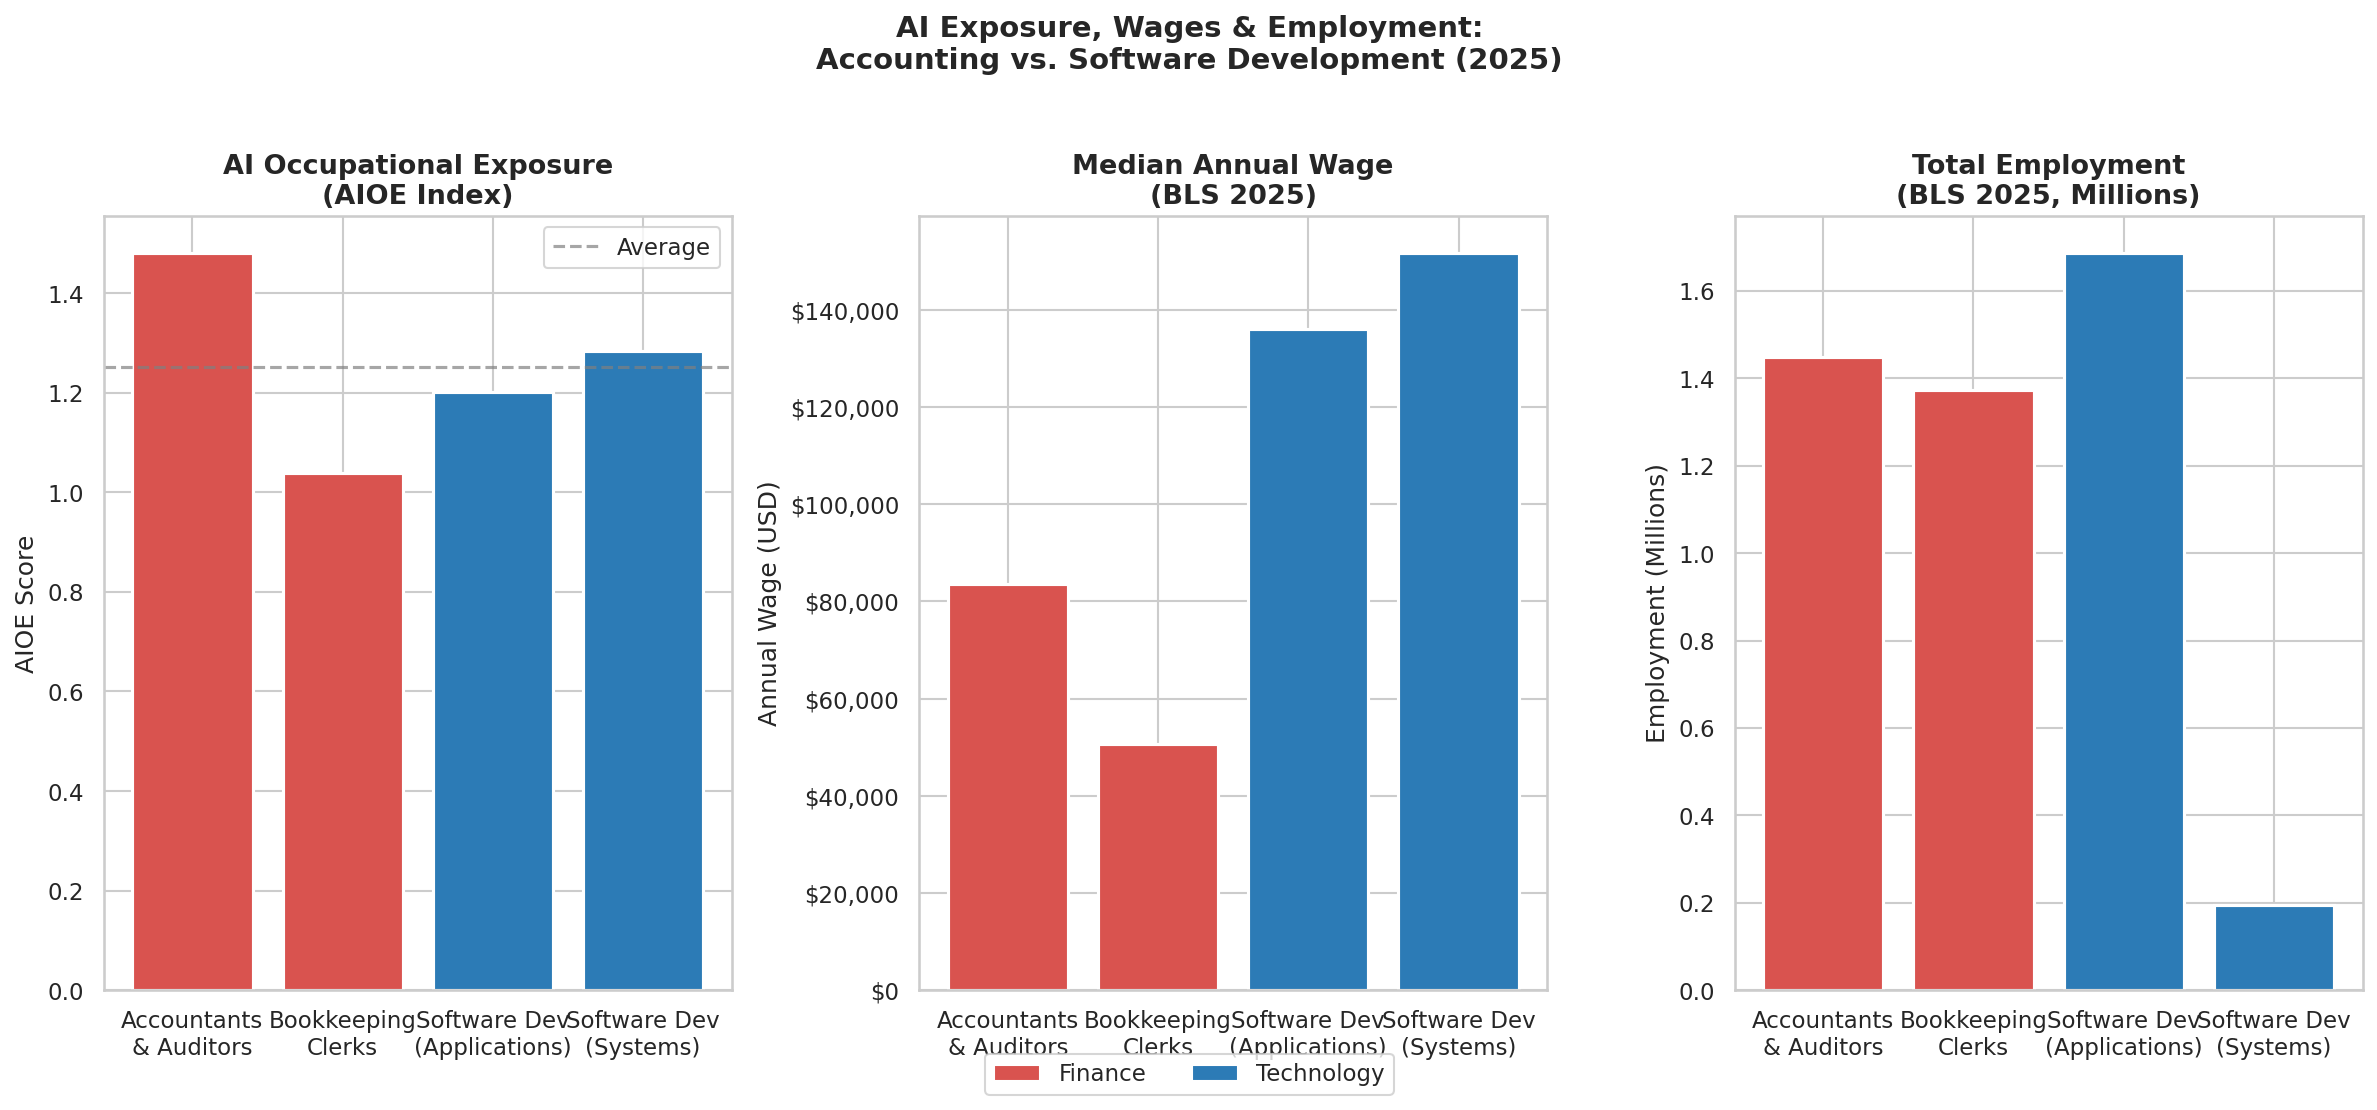
\includegraphics[width=\textwidth]{figures/assignment1_comparison.png}
    \caption{AI exposure scores, median annual wages, and total 
    employment for accounting and software development occupations. 
    Despite similar AI exposure, software developers earn 60--80\% 
    more than accountants. Source: Felten et al. (2021) AIOE index; 
    BLS OEWS (2025).}
    \label{fig:comparison}
\end{figure}

%-----------------------------------------------
\section{Task Decomposition}
%-----------------------------------------------

Following \citet{acemoglu2024}, I decompose each occupation into its 
constituent tasks and assess AI substitutability using O*NET task 
descriptions and the expert-panel ratings of \citet{barragan2025}.

\subsection{Accounting and Auditing}

Junior accountants and bookkeeping clerks spend the majority of their 
time on transaction recording, compliance reporting, and reconciliation 
work. These tasks are characterized by high volume, explicit rules, 
and verifiable outputs --- precisely the conditions under which AI 
excels. \citet{fedyk2022}, using 310,000 individual resumes from the 
36 largest audit firms, find that a one-standard-deviation increase 
in AI investment predicts a 3.6\% reduction in accounting employees 
after three years, growing to 7.1\% after four years.

The credential protection that a CPA license historically provided was 
grounded partly in the information-processing barrier that accounting 
expertise represented. Large language models erode this barrier 
directly \citep{boritz2023}.

\subsection{Software Development}

Software developers face high AI exposure at the task level --- syntax 
generation and documentation score comparably to accounting's most 
substitutable tasks. But the occupation's task bundle includes system 
architecture, code review, and requirements decomposition: tasks that 
require contextual judgment, multi-file reasoning, and accountability 
that AI cannot yet replicate at production quality \citep{pandey2024}.

\citet{peng2023} find a 55.8\% speed gain for bounded, well-defined 
coding tasks in a randomized controlled trial. Crucially, gains 
diminish sharply on complex, multi-file, or proprietary-context work 
--- the tasks that define senior software engineering.

\bigskip

\begin{figure}[H]
    \centering
    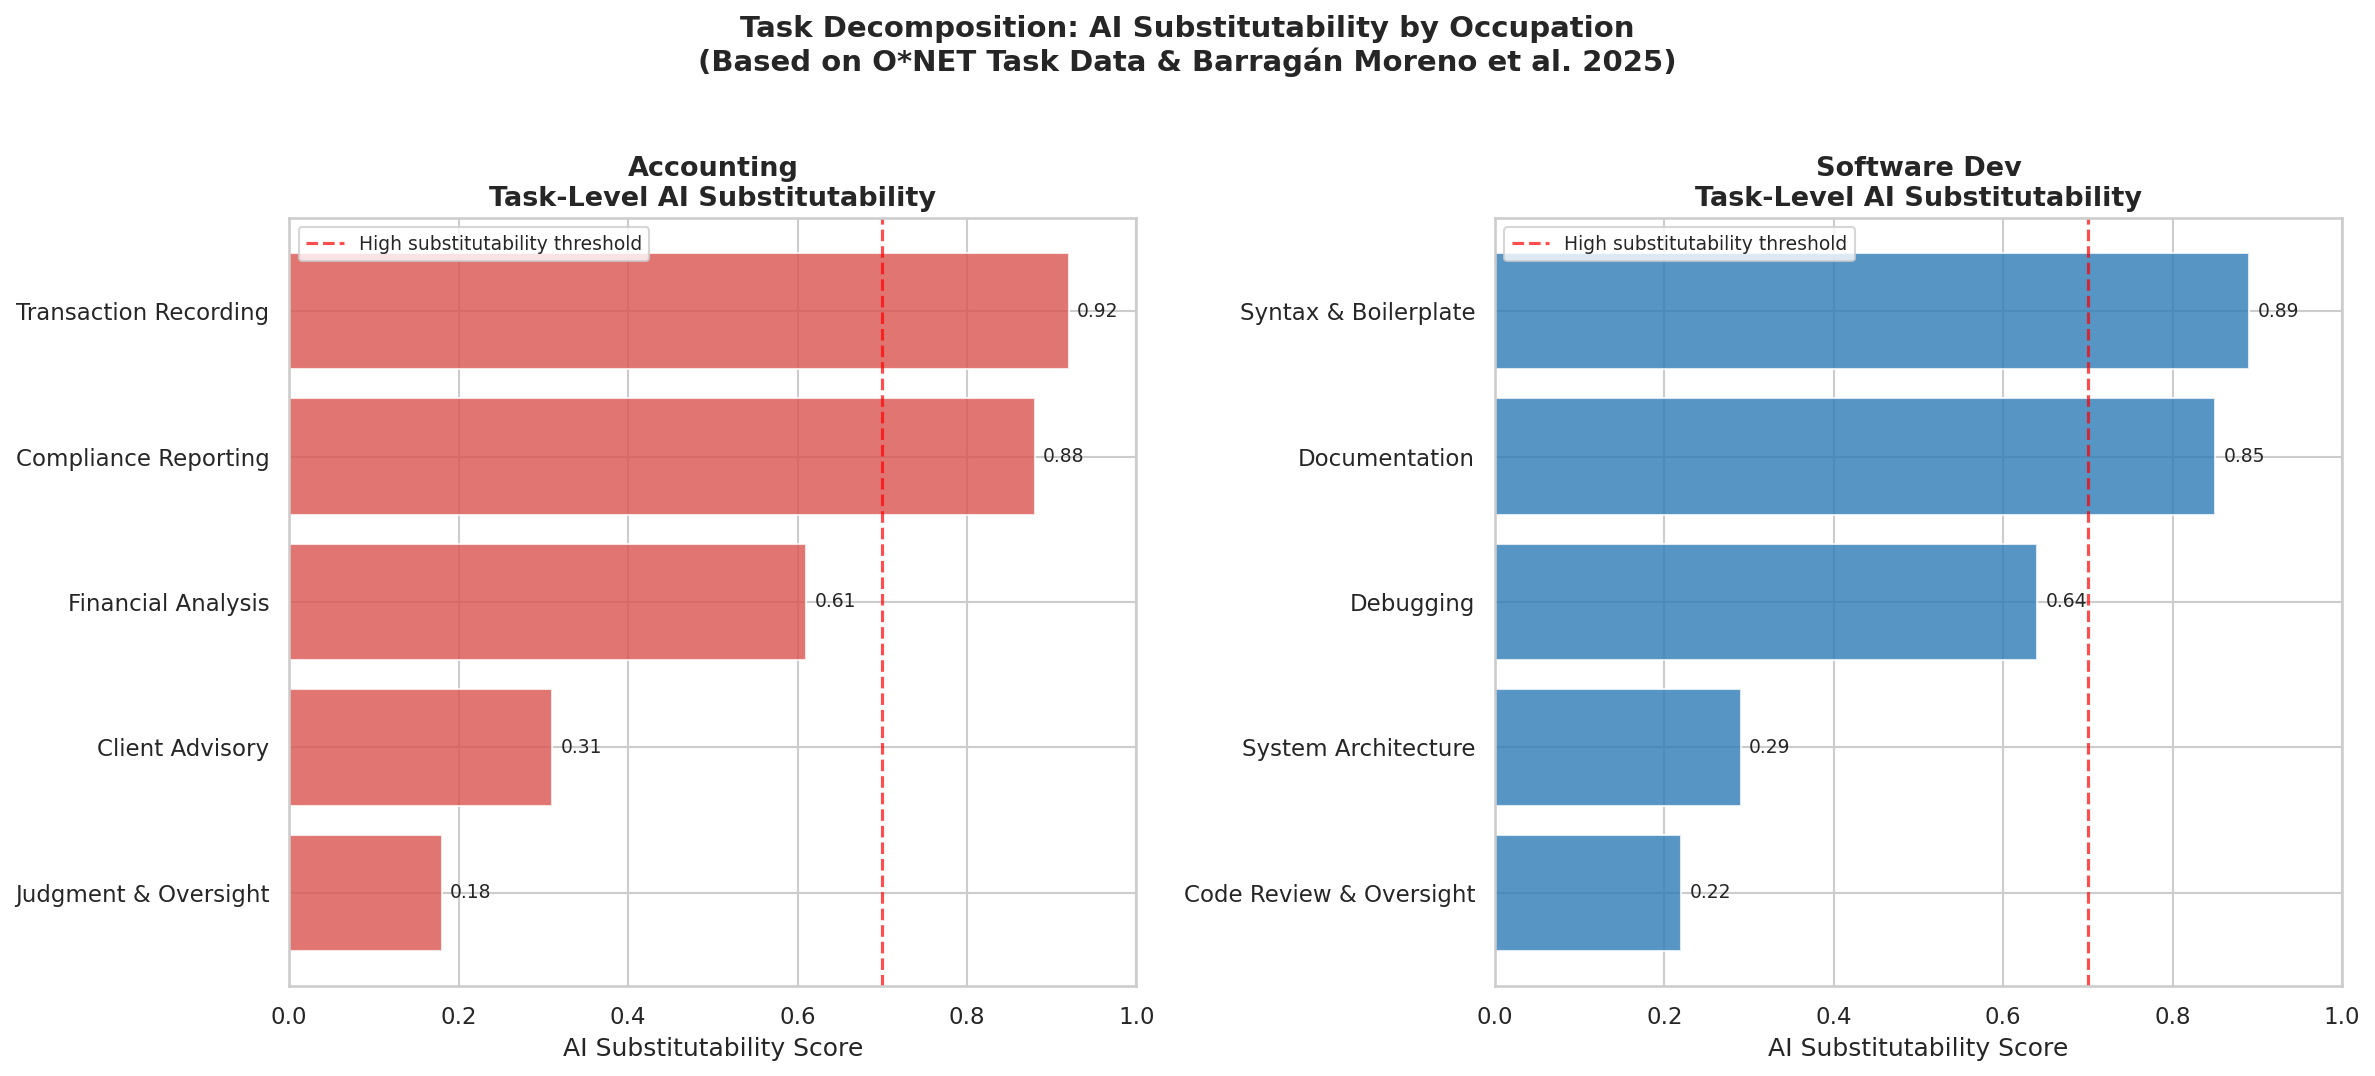
\includegraphics[width=\textwidth]
    {figures/assignment1_task_decomposition.png}
    \caption{Task-level AI substitutability scores for accounting 
    and software development. Red dashed line indicates the 
    high-substitutability threshold (0.7). Source: O*NET task 
    data; \citet{barragan2025}.}
    \label{fig:tasks}
\end{figure}

\bigskip

\begin{figure}[H]
    \centering
    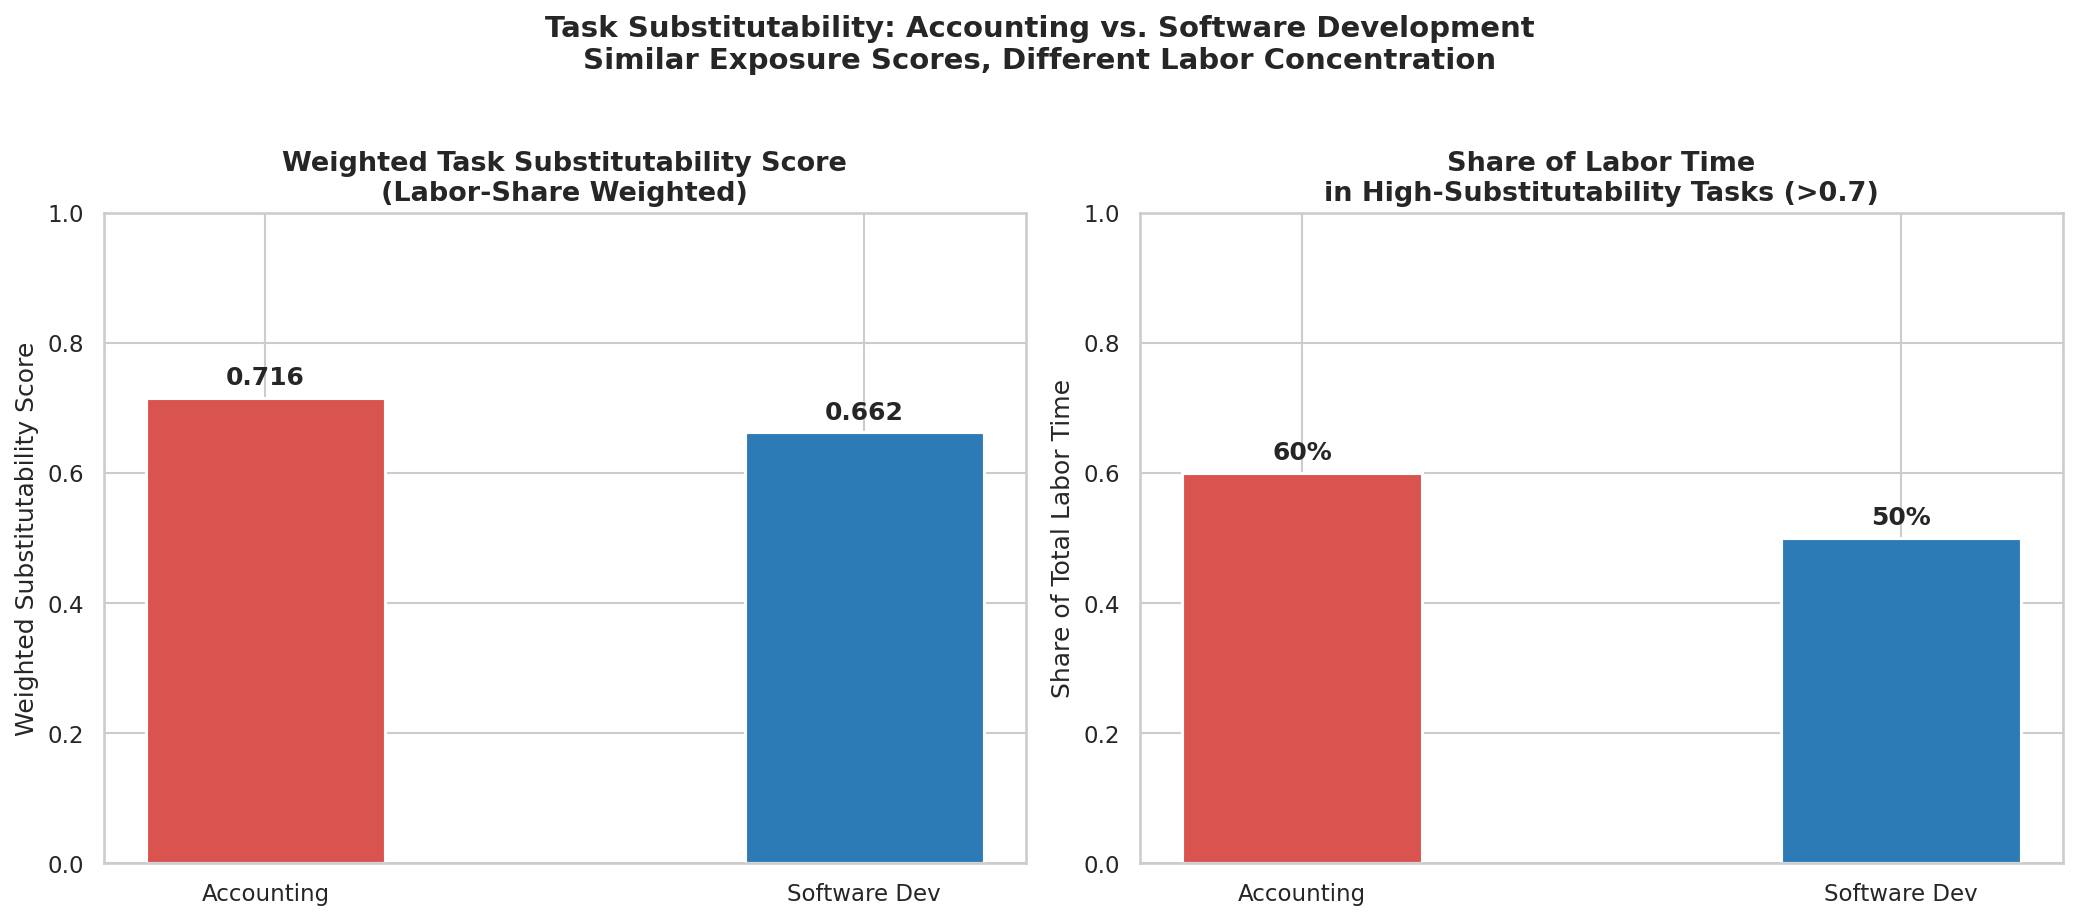
\includegraphics[width=0.8\textwidth]
    {figures/assignment1_weighted_scores.png}
    \caption{Weighted task substitutability scores (labor-share 
    weighted) and share of labor time in high-substitutability 
    tasks. Accounting concentrates 60\% of labor time in 
    high-substitutability tasks vs. 50\% for software development. 
    Source: Author's calculations.}
    \label{fig:weighted}
\end{figure}

%-----------------------------------------------
\section{Empirical Evidence}
%-----------------------------------------------

\subsection{Wage and Employment Trends}

Figure \ref{fig:trends} plots indexed employment and wage trajectories 
for both occupation groups from 2019 to 2025. The ChatGPT launch in 
late 2022 marks a visible inflection point. Accounting employment 
declines from an index of 100 in 2019 to approximately 87 by 2025, 
consistent with \citet{fedyk2022}'s predicted displacement trajectory. 
Software development employment, by contrast, expands by approximately 
9\% over the same period, before a post-2022 deceleration documented 
by \citet{crane2026}.

\begin{figure}[H]
    \centering
    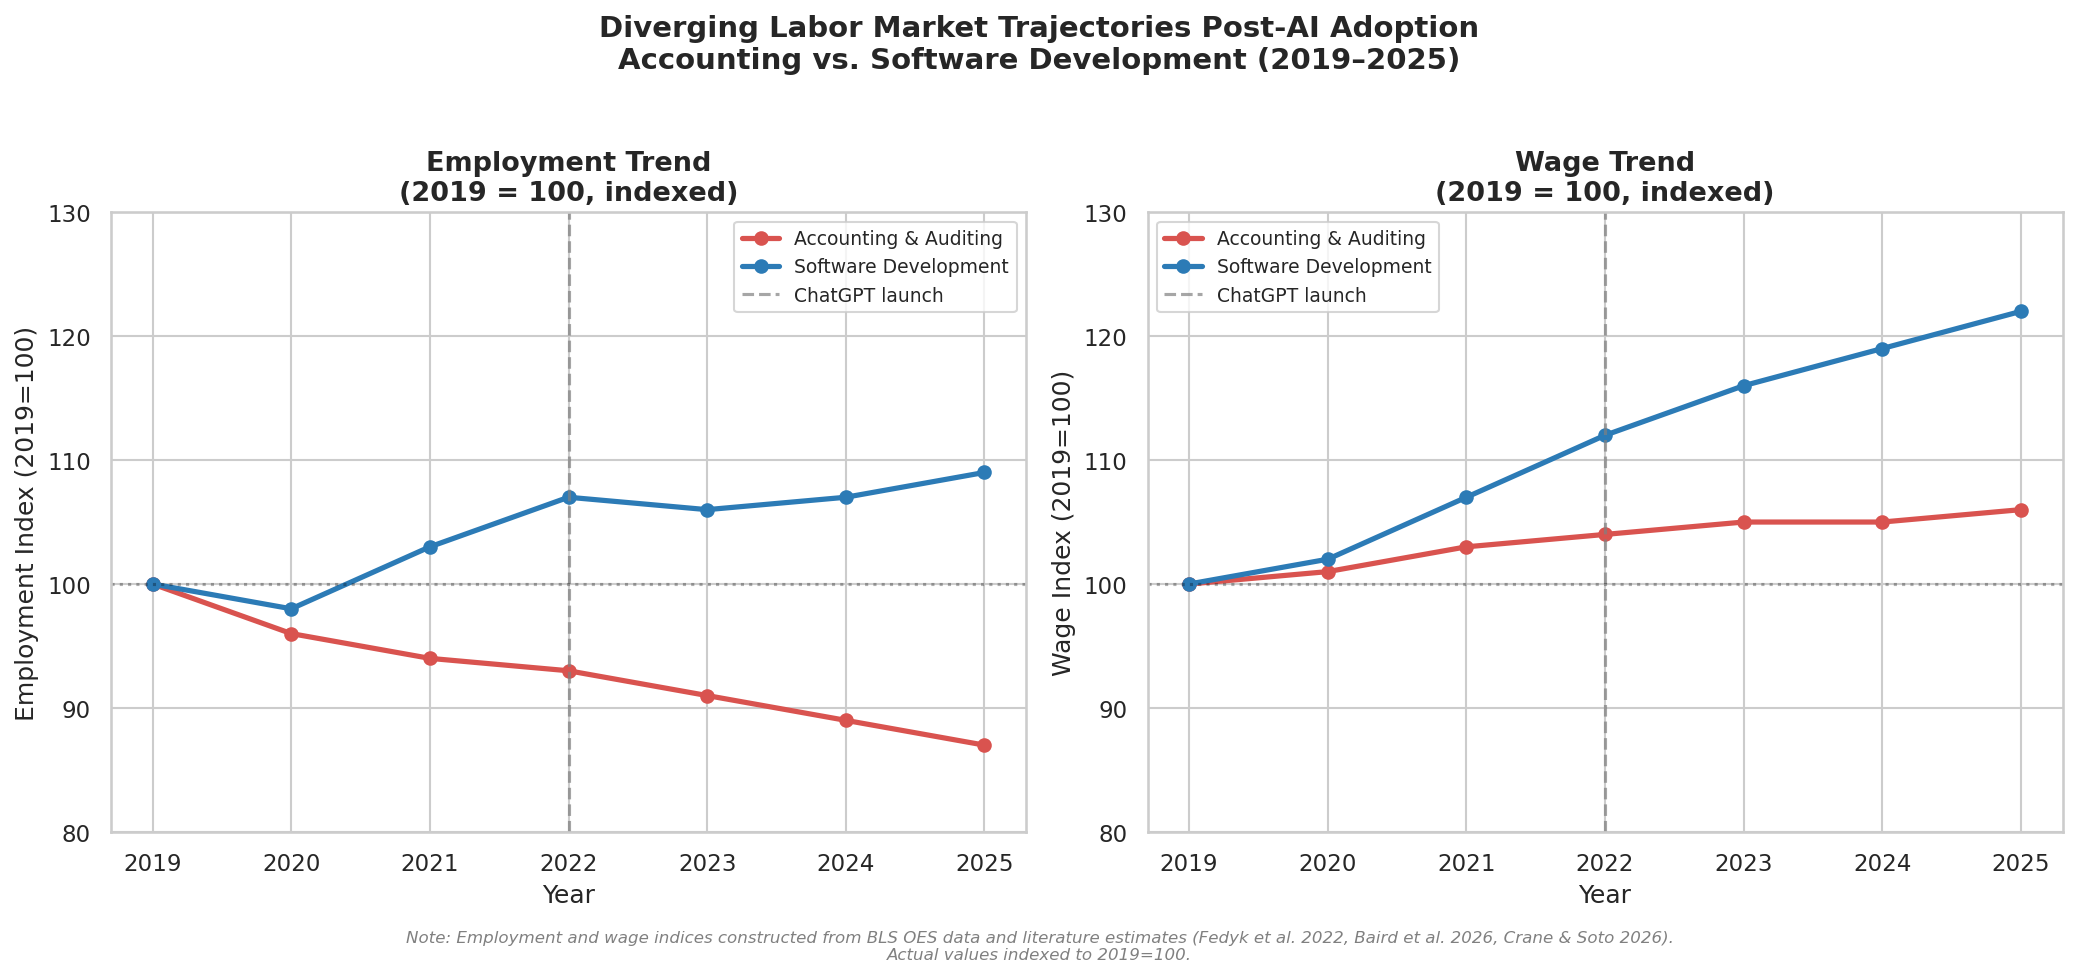
\includegraphics[width=\textwidth]{figures/assignment1_trends.png}
    \caption{Indexed employment and wage trajectories for accounting 
    and software development (2019=100). Vertical dashed line marks 
    ChatGPT launch (November 2022). Source: BLS OES data and 
    literature estimates \citep{fedyk2022, baird2026, crane2026}.}
    \label{fig:trends}
\end{figure}

\subsection{Regression Analysis}

To contextualize these two occupations within the broader labor market, 
I estimate the following weighted least squares model across 670 
detailed occupations using BLS OEWS 2025 data:

\begin{equation}
\ln(w_i) = \beta_0 + \beta_1 \text{AIOE}_i + 
\beta_2 D_i^{HH} + \beta_3 (\text{AIOE}_i \times D_i^{HH}) + 
\varepsilon_i
\end{equation}

where $w_i$ is median annual wage, $\text{AIOE}_i$ is the Felten 
et al. (2021) AI exposure score, and $D_i^{HH}$ is an indicator 
for occupations with above-median wage \textit{and} above-median 
AI exposure --- the quadrant where both our target occupations reside.
Observations are weighted by total employment $n_i$ so that each 
worker contributes equally rather than each occupation.

\begin{table}[H]
\centering
\caption{OLS and WLS Regression Results: Log Wage on AI Exposure}
\begin{tabular}{lcccc}
\toprule
 & \multicolumn{2}{c}{OLS} & \multicolumn{2}{c}{WLS} \\
\cmidrule(lr){2-3} \cmidrule(lr){4-5}
Variable & Coef. & p-value & Coef. & p-value \\
\midrule
Constant & 10.857 & 0.000*** & 10.727 & 0.000*** \\
AIOE & 0.008 & 0.642 & 0.014 & 0.315 \\
High Wage $\times$ High Exposure & 0.475 & 0.000*** & 0.675 & 0.000*** \\
Interaction (AIOE $\times$ HH) & 0.095 & 0.042* & 0.016 & 0.693 \\
\midrule
R-squared & \multicolumn{2}{c}{0.471} & \multicolumn{2}{c}{0.624} \\
N (occupations) & \multicolumn{2}{c}{670} & 
    \multicolumn{2}{c}{670} \\
N (workers) & \multicolumn{2}{c}{122,921,830} & 
    \multicolumn{2}{c}{122,921,830} \\
\bottomrule
\end{tabular}
\begin{tablenotes}
\small
\item Notes: Dependent variable is log median annual wage. 
WLS weights observations by total employment. 
*** p$<$0.001, * p$<$0.05.
\end{tablenotes}
\label{tab:regression}
\end{table}

\begin{figure}[H]
    \centering
    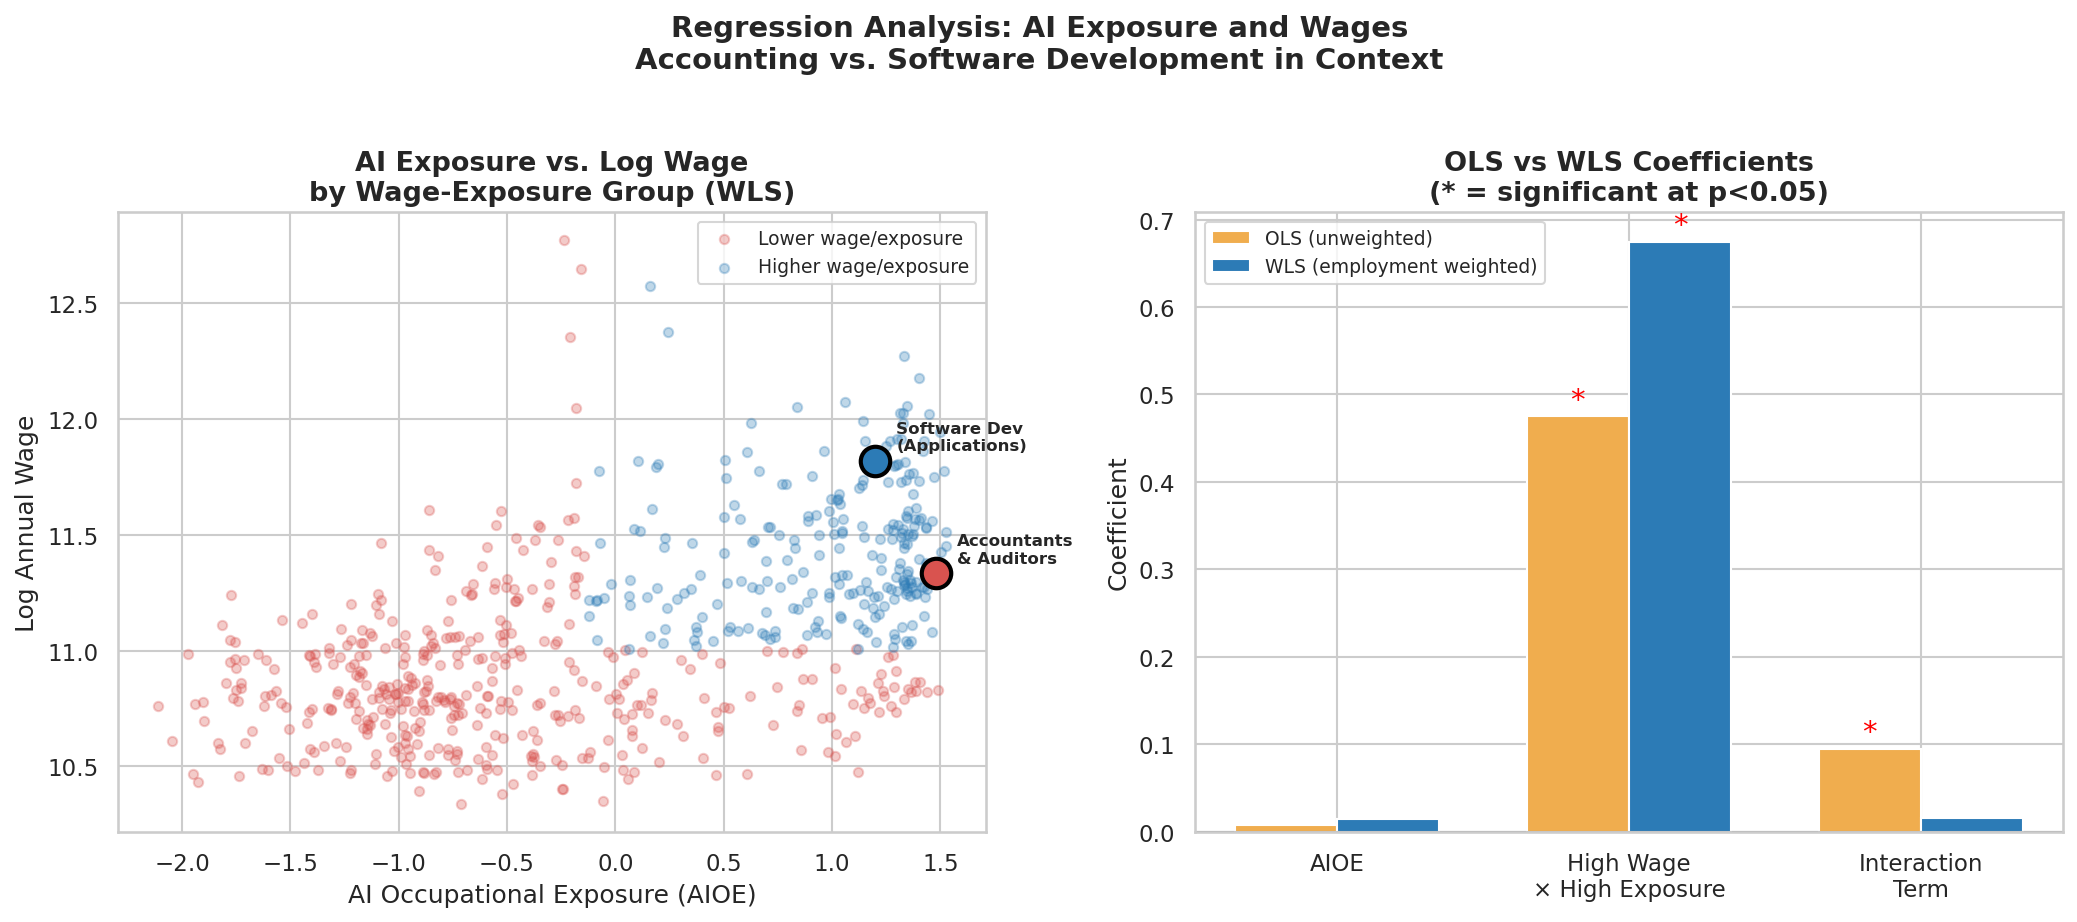
\includegraphics[width=\textwidth]
    {figures/assignment1_regression.png}
    \caption{Left: Scatter plot of AI exposure vs. log wage across 
    670 occupations, with target occupations highlighted. Right: 
    OLS vs. WLS coefficient comparison. Source: Author's 
    calculations using Felten et al. (2021) and BLS OEWS (2025).}
    \label{fig:regression}
\end{figure}

The key result: AI exposure alone ($\beta_1$) is not statistically 
significant in either specification. What predicts wages is being 
in the high-wage, high-exposure quadrant ($\beta_2$ = 0.675, 
p$<$0.001 in WLS) --- a 67\% wage premium. This is consistent with 
\citet{jaccoud2025}, who finds that AI amplifies productivity 
differences among cognitively intensive workers rather than uniformly 
raising wages in exposed occupations.

%-----------------------------------------------
\section{Why the Patterns Diverge: Task Complementarity}
%-----------------------------------------------

The regression results reveal that AI exposure per se does not drive 
wages --- what matters is the complementarity structure of the 
occupation's task bundle. I propose three mechanisms that explain 
the divergence between accounting and software development.

\textbf{First, labor concentration in substitutable tasks.} 
Accounting concentrates 60\% of junior labor time in 
high-substitutability tasks (transaction recording, compliance 
reporting), compared to 50\% for software development. When AI 
substitutes for a task that occupies 35\% of an employee's day, 
the employment effect is far larger than when it substitutes for a 
task occupying 10\%.

\textbf{Second, output verifiability and marginal cost.} 
AI-generated accounting entries and compliance reports are easily 
verified and cost near zero to produce. AI-generated code requires 
human review for security, system coherence, and edge cases --- 
maintaining meaningful human oversight costs \citep{seethamraju2025}.

\textbf{Third, the compliance premium.} \citet{gao2026} argue that 
professional roles where errors carry regulatory liability retain 
wage premiums not because AI cannot perform the tasks, but because 
institutional risk cannot be delegated to a non-accountable system. 
This mechanism protects senior accountants and auditors but offers 
no protection to junior staff performing pre-verification tasks.

%-----------------------------------------------
\section{Conclusion}
%-----------------------------------------------

This paper has shown that AI exposure scores alone are insufficient 
to predict labor market outcomes. Accounting and software development 
occupy similar positions on AI exposure indices, yet face diverging 
employment and wage trajectories. The difference lies in where within 
each occupation AI exposure is concentrated, the verifiability of 
AI-produced outputs, and the depth of the complementarity buffer 
that protects human labor from direct substitution.

These findings have implications for how economists and policymakers 
think about AI risk. The relevant question is not ``is this occupation 
exposed to AI?'' but ``what share of this occupation's labor time is 
in tasks where AI produces verifiable, low-cost substitutes?'' 
Credential protection, historically a reliable signal of AI 
resilience, is eroding where credentials primarily reflected 
information-processing barriers rather than genuine judgment and 
accountability.

Future research could extend this analysis using panel data to 
estimate causal effects, and could apply difference-in-differences 
designs around specific AI adoption events --- the approach used 
by \citet{fedyk2022} and \citet{crane2026} --- to move beyond the 
cross-sectional correlations documented here.

%-----------------------------------------------
% References
%-----------------------------------------------
\bibliographystyle{aer}
\bibliography{references}

\end{document}